\section{Group actions on CAT(0) cube complexes and strong group boundaries}
\label{sec:group}
This chapter is divided in four sections, which themselves cover two general topics. The first two sections deal with group actions of a group \(\Gamma\) on a CAT(0) cube complex \(X\). First, we will convince ourselves that a group action via automorphisms always extends to an action on \(\bar X\) by homeomorphisms. This will be accomplished in Section~\ref{sec:ga-roller}. Then we will introduce two properties for group actions on \(X\), namely \emph{non-elementarity} and \emph{essentiality}. Interestingly, these two properties are rather of a different kind. The first is more concerned with the CAT(0) structure (in particular, the visual boundary) of our space, whereas the second is more concerned with the combinatorial structure of the halfspaces of \(X\).\todo{say more about non-elementarity and essentiality}

The last two sections are concerned with the definition of \emph{strong \(\Gamma\)-boundaries}. First we have a section dedicated to (doubly) ergodic group actions and some elementary consequences (especially concerning the ergodic action of finite groups). In the last section we will generalize the notion of ergodicity to \emph{ergodic group actions with coefficients} and additionally introduce \emph{amenable group actions}. With these two concepts in place, we can finally define a strong group boundary and immediately use it to construct the first half of our boundary map.\todo{say more about strong boundaries}\todo{cite sources for group section}

\subsection{Extending a group action to the Roller boundary}
\label{sec:ga-roller}

In this section we would like to remark on how one can extend a group action on a CAT(0) cube complex \(X\) to its Roller compactification \(\bar X\). For that matter, let \(\Gamma\) be a group with an action \(\Gamma \to \Aut(X)\), where \(X\) is a finite dimensional CAT(0) cube complex. The group \(\Aut(X)\) consists of the combinatorial automorphisms of \(X\) (c.\,.f.\ Def.~\ref{def:morphism-ccc}).

The following proposition collects some facts about how combinatorial isomorphisms act on \(X\). The notation can be found in Section~\ref{sec:halfspaces} and~\ref{sec:roller}.

\begin{prop}
  Let \(g \in \Aut(X)\). Then the following holds:
  \begin{enumerate}
  \item if \(\mathfrak{\hat h} \in \mathcal{\hat H}(X)\) then \( g\mathfrak{\hat h} \in \mathcal{\hat H}(X)\),
  \item if \(\mathfrak{h} \in \mathcal{H}(X)\) then \( g\mathfrak{h} \in \mathcal{H}(X)\),
  \item for every\(\mathfrak{h} \in \mathcal{H}(X)\colon g(\mathfrak{h}^\ast) = (g\mathfrak{h})^\ast\),
  \item if \(\mathfrak{h,h'} \in \mathcal{H}(X)\colon \mathfrak{h} \subset \mathfrak{h'}\) then \(g\mathfrak{h} \subset g\mathfrak{h'}\),
  \item if\(\alpha \in \bar X\) then \(g\alpha \in \bar X\) and
  \item if \(\alpha\) satisfies the descending chain condition then so does \(g\alpha\).
  \end{enumerate}
\end{prop}

\begin{proof}
  The first statement is an immediate consequence of the fact that \(g\) is an isometry. This leads directly to statement 2 and 3. For statement 4 we only need that \(g\) is a bijection. Statements 5 and 6 are then simple applications of 4.
\end{proof}

With the above proposition in place, we see that each group action \(\Gamma \to \Aut(X)\) immediately leads to an action \(\Gamma \to \operatorname{Perm}(\bar X)\). However, this is not yet what we want. We would prefer the image to lie in the homeomorphisms of \(\bar X\). This will be accomplished with the next lemma.

\begin{lemma}
  Let \(g \in \Aut(X)\) and \(\mathcal{U} \coloneqq \mathcal{U}(\mathfrak{h}_1, \dots, \mathfrak{h}_n) \subset \bar X\) a basic open set. Then we have
  \[
    g^{-1} \mathcal{U} = \mathcal{U}(g^{-1}\mathfrak{h}_1, \dots, g^{-1}\mathfrak{h}_n).
  \]
  Hence, \(g \in \operatorname{Homeo}(\bar X)\).
\end{lemma}

Together we arrive at the following result.

\begin{thm}
  \label{thm:roller-action}
  Let \(\Gamma\) be a group and \(\Gamma \to \Aut(X)\) a group action on a CAT(0) cube complex \(X\). Then this action extends to an action \(\Gamma \to \operatorname{Homeo}(\bar X)\) on the Roller compactification.
\end{thm}

\subsection{Non-elementary and essential group actions}
\label{sec:special}

Not every group action on a CAT(0) cube complex leads to our desired boundary map. There are two additionally properties we need to demand in order for our construction to work. These two are introduced in this section. The first is non-elementarity which is concerned with fixed points of the group in \(X\) and in the visual boundary of \(X\) (see Definition~\ref{defin:visual}). The second is essentiality which is concerned with the interplay of the group with the halfspaces \(\mathcal{H}\) of \(X\). The section will close with some results by \textcite{Caprace2010}.

\subsubsection*{Non-elementary group actions}
\label{non-elementary}

\begin{defin}[(Non-)elementary action]
  A group action \(\Gamma \to \Aut(X)\) is called \emph{elementary} if there exists a finite orbit of the action on \(X \sqcup \partial_{\sphericalangle}X\). Otherwise the action is called \emph{non-elementary}.
\end{defin}

The above definition has one interesting immediate consequence:
\begin{prop}
  \label{prop:ne-unbounded}
  If \(\Gamma \to \Aut(X)\) acts non-elementary on \(X\), then the vertex set \(V(X)\) of \(X\) together with the edge metric is unbounded, i.\,e.\ for every \(v \in V(X)\) and every \(K>0\) there exists a \(w \in V(X)\) such that \(d(v,w)>K\). In particular, \(V(X)\) is infinite.
\end{prop}

The previous observation already provides many examples for elementary actions by considering any group action on a finite cube complex. Let us consider an example of a cube complex with infinitely many vertices:

\begin{bsp}[\(\R^d\)]
  Another example is \(X \coloneqq \R^d\) with its standard cubulation and any cyclic subgroup of \(\Z^d\) acting by translations. This action has no finite orbits in \(\R^d\), but every point at infinity is fixed. Indeed, two rays define the same point at infinity if and only if they are parallel. However, a translated ray is still parallel to the untranslated ray.

  As an example for a non-elementary action we consider the universal cover \(\tilde X\) of \(X \coloneqq S^1 \vee S^1\) as depicted in Figure~\ref{fig:figure-8}. The space \(X\) is not a cube complex in our definition, however its universal cover \(\tilde X\) is a tree and hence a CAT(0) cube complex. We let \(\Gamma \coloneqq \operatorname{Deck}(\tilde X/X)\) the group of \emph{deck transformations} (For an introduction to covering space theory and deck transformations see for example~\cite[Section~1.3]{hatcher}). This group acts by combinatorial maps. Indeed, each vertex is mapped to a vertex, since fibers are preserved by deck transformations and each edge is again mapped to an edge (even more: the signing as in Figure~\ref{fig:figure-8} is preserved) because of the path lifting property. 
  \begin{figure}[htbp]
    \centering
    \begin{tikzpicture}
  [
  vertex/.style={
    circle,
    fill=black,
    minimum size=1mm,
    inner sep=0pt
  },
  ->-/.style={
    decoration={
      markings,
      mark=at position 0.5 with {\arrow{#1}}
    },
    postaction={decorate}
  }
  ]

  \node (0) at (0,0) [vertex] {};
  \draw[->] (0,0) arc (0:180: 0.5);
  \draw (0,0) arc (360:180: 0.5);
  \draw[>={Stealth},->] (0,0) arc (0:180:-0.5);
  \draw (0,0) arc (360:180:-0.5);

  \begin{scope}[shift={(5,0)},scale=1.5]
    \node (0) at ( 0, 0) [vertex] {};
    \node (1) at ( 1, 0) [vertex] {};
    \node (2) at ( 0, 1) [vertex] {};
    \node (3) at (-1, 0) [vertex] {};
    \node (4) at ( 0,-1) [vertex] {};
    \draw[->-={>}] (0) -- (1);
    \draw[>={Stealth},->-={>}] (0) -- (2);
    \draw[->-={<}] (0) -- (3);
    \draw[>={Stealth},->-={<}] (0) -- (4);
    \begin{scope}[shift={(0,1)}, scale=0.5]
      \node (0) at ( 0, 0) [vertex] {};
      \node (1) at ( 1, 0) [vertex] {};
      \node (2) at ( 0, 1) [vertex] {};
      \node (3) at (-1, 0) [vertex] {};
      \draw[->-={>[scale=0.5]}] (0) -- (1);
      \draw[>={Stealth},->-={>[scale=0.5]}] (0) -- (2);
      \draw[->-={<[scale=0.5]}] (0) -- (3);
      \begin{scope}[shift={(0,1)}, scale=0.5]
        \node (0) at ( 0, 0) [vertex] {};
        \node (1) at ( 1, 0) [vertex] {};
        \node (2) at ( 0, 1) [vertex] {};
        \node (3) at (-1, 0) [vertex] {};
        \draw[->-={>[scale=0.5]}] (0) -- (1);
        \draw[>={Stealth},->-={>[scale=0.5]}] (0) -- (2);
        \draw[->-={<[scale=0.5]}] (0) -- (3);
        \draw[dotted] (1) -- ( 1.7,0);
        \draw[dotted] (2) -- ( 0,1.7);
        \draw[dotted] (3) -- (-1.7,0);
      \end{scope}
      \begin{scope}[rotate=090,shift={(0,1)},scale=0.5]
        \node (0) at ( 0, 0) [vertex] {};
        \node (1) at ( 1, 0) [vertex] {};
        \node (2) at ( 0, 1) [vertex] {};
        \node (3) at (-1, 0) [vertex] {};
        \draw[>={Stealth},->-={>[scale=0.5]}] (0) -- (1);
        \draw[->-={<[scale=0.5]}] (0) -- (2);
        \draw[>={Stealth},->-={<[scale=0.5]}] (0) -- (3);
        \draw[dotted] (1) -- ( 1.7,0);
        \draw[dotted] (2) -- ( 0,1.7);
        \draw[dotted] (3) -- (-1.7,0);
      \end{scope}
      % \begin{scope}[rotate=180,shift={(0,1)}, scale=0.5]
      %   \node (0) at ( 0, 0) [vertex] {};
      %   \node (1) at ( 1, 0) [vertex] {};
      %   \node (2) at ( 0, 1) [vertex] {};
      %   \node (3) at (-1, 0) [vertex] {};
      %   \draw[->-={<[scale=0.5]}] (0) -- (1);
      %   \draw[>={Stealth},->-={<[scale=0.5]}] (0) -- (2);
      %   \draw[->-={>[scale=0.5]}] (0) -- (3);
      % \end{scope}
      \begin{scope}[rotate=270,shift={(0,1)}, scale=0.5]
        \node (0) at ( 0, 0) [vertex] {};
        \node (1) at ( 1, 0) [vertex] {};
        \node (2) at ( 0, 1) [vertex] {};
        \node (3) at (-1, 0) [vertex] {};
        \draw[>={Stealth},->-={<[scale=0.5]}] (0) -- (1);
        \draw[->-={>[scale=0.5]}] (0) -- (2);
        \draw[>={Stealth},->-={>[scale=0.5]}] (0) -- (3);
        \draw[dotted] (1) -- ( 1.7,0);
        \draw[dotted] (2) -- ( 0,1.7);
        \draw[dotted] (3) -- (-1.7,0);
      \end{scope}
    \end{scope}
    \begin{scope}[rotate=090,shift={(0,1)},scale=0.5]
      \node (0) at ( 0, 0) [vertex] {};
      \node (1) at ( 1, 0) [vertex] {};
      \node (2) at ( 0, 1) [vertex] {};
      \node (3) at (-1, 0) [vertex] {};
      \draw[>={Stealth},->-={>[scale=0.5]}] (0) -- (1);
      \draw[->-={<[scale=0.5]}] (0) -- (2);
      \draw[>={Stealth},->-={<[scale=0.5]}] (0) -- (3);
      \begin{scope}[rotate=270,shift={(0,1)}, scale=0.5]
        \node (0) at ( 0, 0) [vertex] {};
        \node (1) at ( 1, 0) [vertex] {};
        \node (2) at ( 0, 1) [vertex] {};
        \node (3) at (-1, 0) [vertex] {};
        \draw[->-={>[scale=0.5]}] (0) -- (1);
        \draw[>={Stealth},->-={>[scale=0.5]}] (0) -- (2);
        \draw[->-={<[scale=0.5]}] (0) -- (3);
        \draw[dotted] (1) -- ( 1.7,0);
        \draw[dotted] (2) -- ( 0,1.7);
        \draw[dotted] (3) -- (-1.7,0);
      \end{scope}
      \begin{scope}[rotate=000,shift={(0,1)},scale=0.5]
        \node (0) at ( 0, 0) [vertex] {};
        \node (1) at ( 1, 0) [vertex] {};
        \node (2) at ( 0, 1) [vertex] {};
        \node (3) at (-1, 0) [vertex] {};
        \draw[>={Stealth},->-={>[scale=0.5]}] (0) -- (1);
        \draw[->-={<[scale=0.5]}] (0) -- (2);
        \draw[>={Stealth},->-={<[scale=0.5]}] (0) -- (3);
        \draw[dotted] (1) -- ( 1.7,0);
        \draw[dotted] (2) -- ( 0,1.7);
        \draw[dotted] (3) -- (-1.7,0);
      \end{scope}
      \begin{scope}[rotate=090,shift={(0,1)}, scale=0.5]
        \node (0) at ( 0, 0) [vertex] {};
        \node (1) at ( 1, 0) [vertex] {};
        \node (2) at ( 0, 1) [vertex] {};
        \node (3) at (-1, 0) [vertex] {};
        \draw[->-={<[scale=0.5]}] (0) -- (1);
        \draw[>={Stealth},->-={<[scale=0.5]}] (0) -- (2);
        \draw[->-={>[scale=0.5]}] (0) -- (3);
        \draw[dotted] (1) -- ( 1.7,0);
        \draw[dotted] (2) -- ( 0,1.7);
        \draw[dotted] (3) -- (-1.7,0);
      \end{scope}
      % \begin{scope}[rotate=270,shift={(0,1)}, scale=0.5]
      %   \node (0) at ( 0, 0) [vertex] {};
      %   \node (1) at ( 1, 0) [vertex] {};
      %   \node (2) at ( 0, 1) [vertex] {};
      %   \node (3) at (-1, 0) [vertex] {};
      %   \draw[>={Stealth},->-={<[scale=0.5]}] (0) -- (1);
      %   \draw[->-={>[scale=0.5]}] (0) -- (2);
      %   \draw[>={Stealth},->-={>[scale=0.5]}] (0) -- (3);
      % \end{scope}
    \end{scope}
    \begin{scope}[rotate=180,shift={(0,1)}, scale=0.5]
      \node (0) at ( 0, 0) [vertex] {};
      \node (1) at ( 1, 0) [vertex] {};
      \node (2) at ( 0, 1) [vertex] {};
      \node (3) at (-1, 0) [vertex] {};
      \draw[->-={<[scale=0.5]}] (0) -- (1);
      \draw[>={Stealth},->-={<[scale=0.5]}] (0) -- (2);
      \draw[->-={>[scale=0.5]}] (0) -- (3);
      % \begin{scope}[shift={(0,1)}, scale=0.5]
      %   \node (0) at ( 0, 0) [vertex] {};
      %   \node (1) at ( 1, 0) [vertex] {};
      %   \node (2) at ( 0, 1) [vertex] {};
      %   \node (3) at (-1, 0) [vertex] {};
      %   \draw[->-={>[scale=0.5]}] (0) -- (1);
      %   \draw[>={Stealth},->-={>[scale=0.5]}] (0) -- (2);
      %   \draw[->-={<[scale=0.5]}] (0) -- (3);
      % \end{scope}
      \begin{scope}[rotate=270,shift={(0,1)},scale=0.5]
        \node (0) at ( 0, 0) [vertex] {};
        \node (1) at ( 1, 0) [vertex] {};
        \node (2) at ( 0, 1) [vertex] {};
        \node (3) at (-1, 0) [vertex] {};
        \draw[>={Stealth},->-={>[scale=0.5]}] (0) -- (1);
        \draw[->-={<[scale=0.5]}] (0) -- (2);
        \draw[>={Stealth},->-={<[scale=0.5]}] (0) -- (3);
        \draw[dotted] (1) -- ( 1.7,0);
        \draw[dotted] (2) -- ( 0,1.7);
        \draw[dotted] (3) -- (-1.7,0);
      \end{scope}
      \begin{scope}[rotate=000,shift={(0,1)}, scale=0.5]
        \node (0) at ( 0, 0) [vertex] {};
        \node (1) at ( 1, 0) [vertex] {};
        \node (2) at ( 0, 1) [vertex] {};
        \node (3) at (-1, 0) [vertex] {};
        \draw[->-={<[scale=0.5]}] (0) -- (1);
        \draw[>={Stealth},->-={<[scale=0.5]}] (0) -- (2);
        \draw[->-={>[scale=0.5]}] (0) -- (3);
        \draw[dotted] (1) -- ( 1.7,0);
        \draw[dotted] (2) -- ( 0,1.7);
        \draw[dotted] (3) -- (-1.7,0);
      \end{scope}
      \begin{scope}[rotate=090,shift={(0,1)}, scale=0.5]
        \node (0) at ( 0, 0) [vertex] {};
        \node (1) at ( 1, 0) [vertex] {};
        \node (2) at ( 0, 1) [vertex] {};
        \node (3) at (-1, 0) [vertex] {};
        \draw[>={Stealth},->-={<[scale=0.5]}] (0) -- (1);
        \draw[->-={>[scale=0.5]}] (0) -- (2);
        \draw[>={Stealth},->-={>[scale=0.5]}] (0) -- (3);
        \draw[dotted] (1) -- ( 1.7,0);
        \draw[dotted] (2) -- ( 0,1.7);
        \draw[dotted] (3) -- (-1.7,0);
      \end{scope}
    \end{scope}
    \begin{scope}[rotate=270,shift={(0,1)}, scale=0.5]
      \node (0) at ( 0, 0) [vertex] {};
      \node (1) at ( 1, 0) [vertex] {};
      \node (2) at ( 0, 1) [vertex] {};
      \node (3) at (-1, 0) [vertex] {};
      \draw[>={Stealth},->-={<[scale=0.5]}] (0) -- (1);
      \draw[->-={>[scale=0.5]}] (0) -- (2);
      \draw[>={Stealth},->-={>[scale=0.5]}] (0) -- (3);
      \begin{scope}[rotate=090,shift={(0,1)}, scale=0.5]
        \node (0) at ( 0, 0) [vertex] {};
        \node (1) at ( 1, 0) [vertex] {};
        \node (2) at ( 0, 1) [vertex] {};
        \node (3) at (-1, 0) [vertex] {};
        \draw[->-={>[scale=0.5]}] (0) -- (1);
        \draw[>={Stealth},->-={>[scale=0.5]}] (0) -- (2);
        \draw[->-={<[scale=0.5]}] (0) -- (3);
        \draw[dotted] (1) -- ( 1.7,0);
        \draw[dotted] (2) -- ( 0,1.7);
        \draw[dotted] (3) -- (-1.7,0);
      \end{scope}
      % \begin{scope}[rotate=090,shift={(0,1)},scale=0.5]
      %   \node (0) at ( 0, 0) [vertex] {};
      %   \node (1) at ( 1, 0) [vertex] {};
      %   \node (2) at ( 0, 1) [vertex] {};
      %   \node (3) at (-1, 0) [vertex] {};
      %   \draw[>={Stealth},->-={>[scale=0.5]}] (0) -- (1);
      %   \draw[->-={<[scale=0.5]}] (0) -- (2);
      %   \draw[>={Stealth},->-={<[scale=0.5]}] (0) -- (3);
      % \end{scope}
      \begin{scope}[rotate=270,shift={(0,1)}, scale=0.5]
        \node (0) at ( 0, 0) [vertex] {};
        \node (1) at ( 1, 0) [vertex] {};
        \node (2) at ( 0, 1) [vertex] {};
        \node (3) at (-1, 0) [vertex] {};
        \draw[->-={<[scale=0.5]}] (0) -- (1);
        \draw[>={Stealth},->-={<[scale=0.5]}] (0) -- (2);
        \draw[->-={>[scale=0.5]}] (0) -- (3);
        \draw[dotted] (1) -- ( 1.7,0);
        \draw[dotted] (2) -- ( 0,1.7);
        \draw[dotted] (3) -- (-1.7,0);
      \end{scope}
      \begin{scope}[rotate=000,shift={(0,1)}, scale=0.5]
        \node (0) at ( 0, 0) [vertex] {};
        \node (1) at ( 1, 0) [vertex] {};
        \node (2) at ( 0, 1) [vertex] {};
        \node (3) at (-1, 0) [vertex] {};
        \draw[>={Stealth},->-={<[scale=0.5]}] (0) -- (1);
        \draw[->-={>[scale=0.5]}] (0) -- (2);
        \draw[>={Stealth},->-={>[scale=0.5]}] (0) -- (3);
        \draw[dotted] (1) -- ( 1.7,0);
        \draw[dotted] (2) -- ( 0,1.7);
        \draw[dotted] (3) -- (-1.7,0);
      \end{scope}
    \end{scope}
  \end{scope}
\end{tikzpicture}
%%% Local Variables:
%%% mode: latex
%%% TeX-master: "../Master"
%%% End:

    \caption{The pointed sum of two spheres \(X \coloneqq S^1 \vee S^1\) and its universal cover\(\tilde X\). The arrows indicate which edges in the universal cover correspond to which loop in \(X\).}
    \label{fig:figure-8}
  \end{figure}

  The universal cover is always a normal covering. This implies that \(\Gamma\) acts transitively on the vertices. Hence \(\Gamma\) has no finite orbit in \(\tilde X\). Now, consider any geodesic ray \(c\) represented by its vertices \((v_i)_{i \in \N}\). Then each edge \(e_i \coloneqq \overline{v_iv_{i+1}}\) has an assigned signing by an arrow and after translating by a deck transformation, this signing will be the same. Without loss of generality assume that \(e_i\) has signing \tikz{\draw[->] (0,0) -- (0.3,0)}. We choose one of the neighbors \(w_i\) of \(v_i\) such that \(\overline{v_iw_i}\) has signing \tikz{\draw[>={Stealth},->] (0,0) -- (0.3,0)}. Then we choose \(g_i \in \Gamma\) such that \(g_iv_i = w_i\). We claim that \(g_ic\) and \(c\) are not equivalent. Since we can drop any finite number of starting vertices, it satisfies to show the assertion in the case \(i=1\). If \(g_1c\) and \(c\) were equivalent then there exists an \(m \in \N\) such that \(g_1v_m\) is a vertex in \(c\), call it \(v_n\). There is a path connecting the two, namely
  \[
    g_1v_m, g_1v_{m-1}, \dots, g_1v_1, v_1, \dots, v_n.
  \]
  Since we are in a tree, this is the unique path. Hence \(g_1c\) must transverse \(\overline{v_1w_1} = \overline{v_1 (g_1v_1)}\). However, every vertex is at most visited once by \(g_1c\) and its first vertex is \(w_1\). So we need \(m=1\) and \(g_1e_1 = \overline{v_1w_1}\). However, this is impossible, because deck transformations conserve signing of edges. So we established that \(g_ic\) and \(c\) are always inequivalent, showing that any orbit in the visual boundary is infinite.
    % As an example for a non-elmentary action, we consider an infinite complete binary tree \(X\). That means we have a root vertex \(r\) which has exactly two children and each child has again exactly two children and so forth. We consider the group \(\Gamma\) acting on \(X\) generated by the following operations: Reflection and rotation at arbitrary vertices. Reflection switches the two subtrees of a vertex and rotation replaces itself with one of its children and the parent moving further down in the tree. The idea of these generating operations can be found in Figures~\ref{fig:rotation} and~\ref{fig:reflection}.

  % \begin{figure}[htbp]{}
  %   \centering
  %   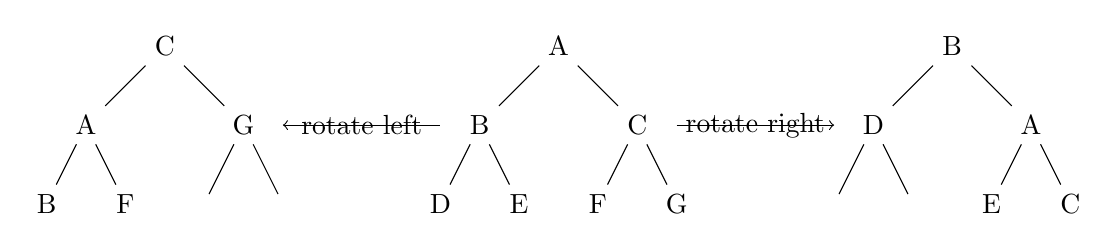
\begin{tikzpicture}
    \node (C'') at ( 0, 0) {C};
    \node (A'') at (-1,-1) {A};
    \node (G'') at ( 1,-1) {G};
    \node (B'') at (-1.5,-2) {B};
    \node (F'') at (-0.5,-2) {F};
    \node (E'') at ( 0.5,-2) {};
    \node (D'') at ( 1.5,-2) {};
    \draw (C'') -- (A'')
    (C'') -- (G'')
    (A'') -- (B'')
    (A'') -- (F'')
    (G'') -- (D'')
    (G'') -- (E'');

    \draw [<-] (1.5,-1) -- node {rotate left} (3.5,-1);
  \begin{scope}[shift={(5,0)}]
  \node (A) at ( 0, 0) {A};
  \node (B) at (-1,-1) {B};
  \node (C) at ( 1,-1) {C};
  \node (D) at (-1.5,-2) {D};
  \node (E) at (-0.5,-2) {E};
  \node (F) at ( 0.5,-2) {F};
  \node (G) at ( 1.5,-2) {G};
  \draw (A) -- (B);
  \draw (A) -- (C);
  \draw (B) -- (D)
  (B) -- (E)
  (C) -- (F)
  (C) -- (G);
  \draw [->] (1.5,-1) -- node {rotate right} (3.5,-1);
  \begin{scope}[shift={(5,0)}]
    \node (B') at ( 0, 0) {B};
    \node (D') at (-1,-1) {D};
    \node (A') at ( 1,-1) {A};
    \node (F') at (-1.5,-2) {};
    \node (G') at (-0.5,-2) {};
    \node (E') at ( 0.5,-2) {E};
    \node (C') at ( 1.5,-2) {C};
    \draw (B') -- (D')
    (B') -- (A')
    (A') -- (E')
    (A') -- (C')
    (D') -- (F')
    (D') -- (G');
  \end{scope}
    
  \end{scope}

\end{tikzpicture}

%%% Local Variables:
%%% mode: latex
%%% TeX-master: "../Master"
%%% End:

  %   \caption{Rotation of a binary (sub-)tree}
  %   \label{fig:rotation}
  % \end{figure}

  % \begin{figure}[htbp]
  %   \centering
  %   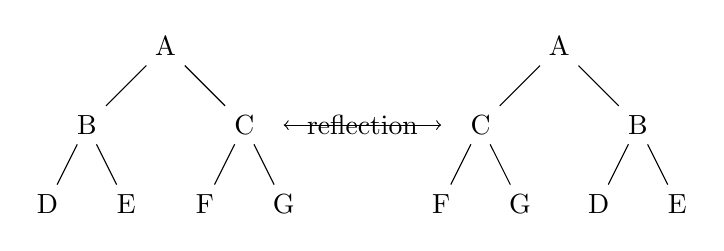
\begin{tikzpicture}
  \node (A) at (0,0) {A};
  \node (B) at (-1,-1) {B};
  \node (C) at ( 1,-1) {C};
  \node (D) at (-1.5,-2) {D};
  \node (E) at (-0.5,-2) {E};
  \node (F) at ( 0.5,-2) {F};
  \node (G) at ( 1.5,-2) {G};
  \draw
  (A) -- (B)
  (A) -- (C)
  (B) -- (D)
  (B) -- (E)
  (C) -- (F)
  (C) -- (G);
  \draw[<->] (1.5,-1) -- node {reflection} (3.5,-1);
  \begin{scope}[shift={(5,0)}]
  \node (A') at (0,0) {A};
  \node (B') at ( 1,-1) {B};
  \node (C') at (-1,-1) {C};
  \node (D') at ( 0.5,-2) {D};
  \node (E') at ( 1.5,-2) {E};
  \node (F') at (-1.5,-2) {F};
  \node (G') at (-0.5,-2) {G};
  \draw
  (A') -- (B')
  (A') -- (C')
  (B') -- (D')
  (B') -- (E')
  (C') -- (F')
  (C') -- (G');
  \end{scope}
\end{tikzpicture}

%%% Local Variables:
%%% mode: latex
%%% TeX-master: "../Master"
%%% End:

  %   \caption{Reflection of a binary (sub-)tree}
  %   \label{fig:reflection}
  % \end{figure}
  % We first check, that we have no finite orbit in \(X\) itself. This can be established via the rotation. Taking any vertx \(v\) we can rotate around this vertex multiple times and with each one the original \(v\) will be pushed deeper down the tree. Hence, every orbit contains infinitely many points. In order to see that there are no finite orbits at infinity, we need to check when to geodesic rays have bounded distance from one another. However, in a tree this is only the case if they coincide after finitely many steps. Hence, every geodesic ray has a unique representative emanating from the root \(r\). Choosing any such geodesic ray, we can generate infinitely many inequivalent ones by reflecting at vertices traversed by it, showing again that there is no finite orbit.
\end{bsp}

\subsubsection*{Essential group actions}
\label{sec:essential}

\begin{defin}[The essential core]
  A halfspace \(h \in \mathcal{H}\) is called \emph{\(\Gamma\)-essential} if for some \(x \in X\) the orbit in \(h\), \(\Gamma x \cap h\), is \emph{not} a bounded distance away from \(\hat h\). A hyperplane \(\hat h \in \mathcal{\hat H}\) is called \emph{\(\Gamma\)-essential} if both its halfspaces are \(\Gamma\)-essential. It is called \emph{half-essential} if only one of its halfspaces is \(\Gamma\)-essential.

  \(\Ess(X,\Gamma)\subset \mathcal{\hat H}(X)\) denotes the set of all essential hyperplanes. Accordingly, \(\nEss(X,\Gamma) \subset \mathcal{\hat H}(X)\) denotes the set of all non-essential hyperplanes, leading to
  \[
    \mathcal{\hat H}(X) = \Ess(X, \Gamma) \sqcup \nEss(X, \Gamma).
  \]
\end{defin}

The above definition leads to the following consequence:

\begin{prop}
  The sets \(\Ess(X, \Gamma)\) and \(\nEss(X, \Gamma)\) are \(\Gamma\)-invariant.
\end{prop}

\begin{defin}
  The \emph{essential core} is the CAT(0) cube complex corresponding to the the pocset of halfspaces \(\Ess(X, \Gamma)\).
\end{defin}

\begin{prop}[{\cite[Proposition~3.5]{Caprace2010}}]
  \label{prop:cs-3.5}
  Let \(X\) be a finite-dimensional CAT(0) cube complex and let \(\Gamma \leq \Aut(X)\). Assume that at least one of the following two conditions is satisfied:
  \begin{enumerate}
  \item \(\Gamma\) has finitely many orbits of hyperplanes or
  \item \(\Gamma\) has not fixed point at infinity.
  \end{enumerate}
  Then the essential core of \(X\) is unbounded if and only if \(\Gamma\) has no fixed point. In that case the essential core embeds as a \(\Gamma\)-invariant convex subcomplex \(Y\) of \(X\).
\end{prop}

\begin{rem}
  Even if \(X\) is irreducible the same might not be true for the essential core \(Y\). \todo{find counterexample for reducible essential core}
\end{rem}

\begin{defin}[Essential action]
  A group action \(\Gamma \to \Aut(X)\) is called \emph{essential} if the essential core of \(\Gamma\) is the whole space \(X\).
\end{defin}

\begin{bsp}
  Consider \(X\coloneqq \R^d\) with the standard cubulation and the action of \(\Gamma \coloneqq \Z^d\) on it via translations. This action respects the cube complex structure. Additionally, every hyperplane in \(X\) is a hyperplane \(\mathfrak{\hat h} \in \mathcal{\hat H}(X)\) in the usual Euclidean sense. The translates of any vertex get arbitrarily far away from \(\mathfrak{h}\) on either side. Hence \(\Gamma\) acts essentially on \(X\).
\end{bsp}

\begin{lemma}[{\cite[Lemma~2.28]{MR3509968}}]
  \label{lem:2.28}
  Let \(X\) be a finite dimensional CAT(0) cube complex and let \(\Gamma \to \Aut(X)\) be a non-elementary action. Then the \(\Gamma_0\)-action on the irreducible factors of the essential core is also non-elementary and essential, where \(\Gamma_0\) is the finite index subgroup preserving the decomposition in irreducible factors.
\end{lemma}

\begin{proof}
  Let \(Y \subset X\) be the essential factor and \(Y = Y_1 \times \dots \times Y_m\) its decomposition into irreducible factors. Let \(\Gamma_0\) be the finite index subgroup of \(\Gamma\) preserving this decomposition.

  We will first show that the \(\Gamma_0\)-action on each \(Y_i\) is essential. By construction \(\Gamma\) acts essentially on \(Y\) and since \(\Gamma_0\) has finite index in \(\Gamma\) the same is true for \(\Gamma_0\). We would like to apply Lemma~\ref{lem:ess-unbounded}. For this we note that any halfspace \(\mathfrak{h}_i \in \mathcal{\hat H}(Y_i)\) defines a unique halfspace in \(Y\) via
  \[
    \mathfrak{h} \coloneqq Y_1 \times \dots \times Y_{i-1} \times \mathfrak{h}_i \times Y_{i+1} \times \dots \times Y_k.
  \]
  Using this each hyperplane \(\mathfrak{\hat h}_i = \{\mathfrak{h}_i , \mathfrak{h}_i^\ast\} \in \mathcal{\hat H}(Y_i)\) defines an associated hyperplane \(\mathfrak{\hat h} = \{\mathfrak{h}, \mathfrak{h}^\ast\}\). Since \(\Gamma_0\) acts essentially on \(Y\), Lemma~\ref{lem:ess-unbounded} assures us that there exists \(g \in \Gamma_0\) and \(n \in \N\) such that \(g^n \mathfrak{h} \subsetneq \mathfrak{h}\) (after possibly switching \(\mathfrak{h}\) and \(\mathfrak{h}^\ast\)). We have \(g^n \mathfrak{h}_i \subsetneq \mathfrak{h}_i\) and using the same lemma in the other direction, we yield that \(\Gamma_0\) acts essentially on each \(Y_i\).

  Secondly, we will show that \(Y_i\) does not have a fixed point as infinity. We will achieve this by contraposition. Assume that \(\Gamma_0 \leq \Gamma\) has a finite orbit. Passing to a further finite index subgroup, which we will still call \(\Gamma_0\), we can assume that \(\Gamma_0\) has a fixed point at infinity. However, then we can apply Lemma~\ref{lem:2.9} and see that we have a \(\Gamma_0\)-fixed point in \(\partial_\sphericalangle Y \subset \partial_\sphericalangle X\). By the finite index, \(\Gamma\) must have a finite orbit at infinity.
\end{proof}

\subsubsection*{Consequences of non-elementary and essential group actions}
\label{cons-non-el-ess}

This paragraph contains some consequences and chracterizations of non-elementary and essential group actions. All of these have been found by \textcite{Caprace2010} and we refer the reader to this text for the proofs.

\begin{lemma}[{\cite[Proposition~3.2]{Caprace2010}}]
  \label{lem:ess-unbounded}
  Let \(X\) be a finite dimensional CAT(0) cube complex, \(\mathfrak{\hat h} \in \mathcal{\hat H}(X)\) and \(\Gamma \leq \Aut(X)\). Then the following are equivalent
  \begin{enumerate}
  \item \(\mathfrak{\hat h} \in \Ess(X,\Gamma)\),
  \item  \(X(\Gamma \cdot \mathfrak{\hat h})\) is unbounded and
  \item \(\Gamma\) \emph{skewers} \(\mathfrak{\hat h}\), i.\,e.\ there exists \(g \in \Gamma\) and \(n \in \N\) such that for one \(\mathfrak{h}\) of the two halfspaces of \(\mathfrak{\hat h}\) we have \(g^n \mathfrak{h} \subsetneq \mathfrak{h}\).
  \end{enumerate}
\end{lemma}

\begin{lemma}[{\cite[Double Skewering Lemma]{Caprace2010}}]
  \label{lem:cs-dsl}
  Let \(X\) be a finite-dimensional CAT(0) cube complex and \(\Gamma \leq \Aut(X)\) be a group acting essentially and without fixed point at infinity. Then for any two halfspaces \(\mathfrak{k} \subset \mathfrak{h}\), there exists \(g \in \Gamma\) such that \(g \mathfrak{h} \subsetneq \mathfrak{k} \subset \mathfrak{h}\).
\end{lemma}

\begin{thm}[{\cite[Theorem~4.1]{Caprace2010}}]
  \label{thm:cs-flipping}
  Assume that \(X\) is a finite-dimensional CAT(0) cube complex and let \(\Gamma \leq \Aut(X)\) be any subgroup. Let \(\mathfrak{h} \in \mathcal{H}(X)\) such that \(\mathfrak{h}^\ast \not\subset g\mathfrak{h}\) for each \(g \in \Gamma\). Then \(\Gamma\) has a fixed point in the visual boundary or \(\mathfrak{h}\) is not essential with regard to \(\Gamma\).
\end{thm}

\begin{prop}[{\cite[Proposition~5.1]{Caprace2010}}]
  \label{prop:cs-5.1}
  Let \(X\) be a finite-dimensional unbounded CAT(0) cube complex such that \(\Aut(X)\) acts essentially and without fixed point at infinity. Then the following conditions are equivalent:
  \begin{enumerate}
  \item \(X\) is irreducible.
  \item There is a pair of strongly separated hyperplanes.
  \item For each halfspace \(\mathfrak{h}\) there is a pair of strongly separated halfspaces \(\mathfrak{h_i}\) such that \(\mathfrak{h}_1 \subset \mathfrak{h} \subset \mathfrak{h}_2\).
  \end{enumerate}
\end{prop}


\subsection{(Doubly) ergodic group actions}
\label{sec:ergodic}

We not only need certain properties of our group action on our complex, but also on its so called strong boundary (which will be introduced in the next section). One of these properties is \emph{ergodicity}. We will mostly use it to make certain maps essentially constant. One other guise we need it in is that ergodic actions of finite groups lead to purely atomic spaces (c.\,f.\ Definition~\ref{defin:atomic} and Lemma~\ref{lem:ergodic-atomic}). Lastly, we will introduce \emph{standard Borel} and \emph{Lebesgue spaces} and prove one last technical lemma making use of this definition and Mackey's point realization (Theorem~\ref{thm:mackey}).

Unless noted otherwise, \(\Gamma\) will denote a countable, discrete group.

\begin{defin}[Measure class preserving action]
  Let \((B, \Sigma)\) be a measurable space. We can define an equivalence relation on all measures on \(\Sigma\) via \(\mu \sim \nu\) if and only if the null-sets of \(\mu\) and \(\nu\) coincide. An equivalence class \([\mu]\) is called a \emph{measure class}. If a group \(\Gamma\) acts by measurable transformations on \(B\), then \(\Gamma\) \emph{preserves measure classes} if for every measure \(\mu\) of \(\Sigma\) we have that \(\mu(B) = 0\) implies that \(\mu(g^{-1} B) = 0\) for every \(B \in \Sigma\) and \(g \in \Gamma\).
\end{defin}

\begin{lemma}
  \label{lem:countable-orbit}
  Let \((M, \Sigma, \mu)\) be a measure space on which a countable group \(\Gamma\) acts by measurable and measure class preserving transformations. Let \(B \in \Sigma\) such that \(\mu(M \setminus B) = 0\). Then there exists \(x \in M\) such that \(\Gamma \cdot x \subset B\).
\end{lemma}

\begin{proof}
  We define
  \[
    A \coloneqq \{x \in B \mid \exists g \in \Gamma\colon gx \in B^c\} = B \cap \left( \bigcup_{g \in \Gamma} gB^c\right) \subset \bigcup_{g \in \Gamma} gB^c.
  \]
  Since \(\Gamma\) acts measure class preserving, we have that \(\mu(gB^c) = 0\) for every \(g \in \Gamma\). As \(\Gamma\) is countable, we have that \(\mu(A) = 0\). Hence \(B \setminus A\) has full measure. In particular it is not empty and every \(x \in B \setminus A\) satisfies \(\Gamma \cdot x \subset B\).
\end{proof}

\begin{defin}[(Doubly) ergodic action]
  Let \((B, \Sigma, \mu)\) be a probability space with a group \(\Gamma\) acting by measurable and measure preserving transformations. Then the action is called \emph{ergodic} if one of the two equivalent conditions is satisfied (c.\,f.\ the following lemma):
  \begin{enumerate}
  \item For every \(E \in \Sigma\) such that \(g^{-1}E = E\) for each \(g \in \Gamma\) we have \(\mu(E) = 0\) or \(\mu(E) = 1\);
  \item every measurable \(\Gamma\)-invariant map \(f\colon B \to \R\) is essentially constant.
  \end{enumerate}
  The action is called \emph{doubly ergodic} if the diagonal action on \(B \times B\) equipped with the product measure is ergodic.
\end{defin}

\begin{lemma}
  The two statements in the above definition are equivalent.
\end{lemma}

\begin{proof}
  We assume 1.\ and we will prove 2. Let \(f \colon B \to \R\) be measurable and \(\Gamma\)-invariant. Then for every \(c \in \R\), we have \(f^{-1}(c)\) is a measurable \(\Gamma\)-invariant set. Hence, it has either measure 0 or 1. Since \(B\) is a disjoint union of all these preimages, we see that there exists exactly one \(c \in \R\) such that \(f^{-1}(c)\) has full measure, which means that \(f\) is essentially constant.

  Now, we will assume 2.\ and we will prove 1. Consider a \(\Gamma\)-invariant measurable set \(E\). Then its indicator function \(\chi_E\) is a measurable, \(\Gamma\)-invariant map and hence essentially constant implying \(\mu(E) \in \{0,1\}\).
\end{proof}

The first definition of ergodicity shows that \emph{transitive} group actions (i.\,e.\ for every \(x,y \in B\) there exists a \(g \in \Gamma\) such that \(gx = y\)) are automatically ergodic (as long as they act measurably and measure class preserving). The following is a less pathological example:

\begin{bsp}[Bernoulli space]
  Consider the Bernoulli space \(B \coloneqq \{0,1\}^{\Z}\) with the product \(\sigma\)-algebra stemming from the discrete topology on each of the sets \(\{0,1\}\). We equip this space with the measure \(\mu\) that comes from the uniform distribution on each factor. Let \(\Z\) act on this space via a shift operation. Then \textcite[Example 20.26]{Klenke} shows that this system is ergodic.
\end{bsp}

\begin{prop}
  \label{prop:coeff-ergodic}
  Every doubly ergodic action is ergodic.
\end{prop}

\begin{proof}[Sketch]
  Consider the second criterion together with the (equivariant, measurable and non-constant) projection from the product to the first factor.
\end{proof}

\begin{lemma}
  \label{lemma:ergodicity-pushforward}
  Let \(A\) and \(B\) be measurable spaces with a measurable group action \(\Gamma\). Furthermore, let \(f\colon A \to B\) be a measurable \(\Gamma\)-equivariant map and \(\mu\) a measure on \(A\). If \(\Gamma\) acts ergodically on \((A, \mu)\) then \(\Gamma\) acts ergodically on \((B, f_\ast \mu)\), where \(f_\ast \mu\) is the pushforward measure (see Definition~\ref{defin:pushforward}).
\end{lemma}

\begin{proof}
  We will apply the first criterion for ergodicity. Let \(E \subset B\) be measurable such that \(g^{-1} E = E\) for every \(g \in \Gamma\). Then we have:
  \[
    f^{-1}(E) = f^{-1}(g^{-1}E) = g^{-1}f^{-1}(E)
  \]
  because of the equivariance. Thus by the ergodicity on \(A\) we have \(\mu(f^{-1}(E))= 0\) or \(\mu(f^{-1}(E)) = 1\). However, \(\mu(f^{-1}(E))\) is exactly the definition of \(f_\ast\mu(E)\).
\end{proof}

\begin{defin}
  \label{defin:atomic}
  Let \((M, \Sigma, \mu)\) be a measure space. A set \(B \in \Sigma\) is called \emph{atomic} if \(\mu(B) > 0\) and for all measurable \(A \subset B\) either \(\mu(A) = 0\) or \(\mu(A) = \mu(B)\). The space \(M\) is \emph{purely atomic} if there exists a partition of \(M\) consisting atomic sets.
\end{defin}

\begin{lemma}
  \label{lem:ergodic-atomic}
  Let \((M, \Sigma, \mu)\) be a measure space and \(\Gamma\) a finite group acting ergodically on it. Then \(M\) is purely atomic.
\end{lemma}

\begin{proof}
  We will find the above mentioned partition. Start by considering the following set:
  \[
    \Lambda \coloneqq \{A \in \Sigma \mid \mu(A) > 0\}.
  \]
  This set is clearly partially ordered under inclusion and not empty. Now, observe that for each \(A \in \Sigma\) such that \(\mu(A) > 0\), we have that \(\mu(\Gamma \cdot A) = 1\) by ergodicity. Since \(\Gamma\) also preservs measures \(\mu(A) > n^{-1}\), where \(n \coloneqq |\Gamma|\). Thus we can rewrite \(\Lambda\) as
  \[
    \Lambda = \{A \in \Sigma \mid \mu(A) \geq n^{-1}\}.
  \]
  Next consider a descending chain \(A_1 \supset A_2 \supset A_3 \supset \dots\) in \(\Lambda\). Then \(A \coloneqq \cap_i A_i\) is also measurable, and since
  \[
    \mu\left(\bigcap_{i=1}^k A_i \right) = \mu(A_k) \geq \frac1n
  \]
  we have \(\mu(A) \geq n^{-1}\) and \(A\) lies in \(\Lambda\). Thus we have found a lower bound for our chain. Applying Zorn's Lemma we find a minimal element \(A \in \Lambda\), i.\,e.\ for every \(B \in \Lambda\) such that \(B \subset A\) we have \(B = A\). Observe that for each \(g \in \Gamma\), the set \(gA\) is also a minimal element. Indeed, if \(B \subset gA\) then \(g^{-1} B \subset A\). Hence \(g^{-1}B = A\) and multiplying again we find \(B = gA\).

  Let us consider the case that \(A\) is \(\Gamma\)-invariant. Then by ergodicity, we have \(\mu(A) = 1\). We claim that in this case \(M\) is atomic. Take any \(B \in \Sigma\).
  Then
  \[
    \mu(B) = \mu(B \cap A) + \mu(B \cap A^c) = \mu(B \cap A),
  \]
  since \(A^c\) is a null-set. We see that \(B \cap A \subset A\) and thus either \(\mu(B \cap A) = 0\) or \(B  \cap A \in \Lambda\) and hence \(B \cap A = A\) and \(\mu(B) = 1 = \mu(M)\).

  If \(A\) is not \(\Gamma\)-invariant, we can consider the sets \(A \cap gA\) for each \(g \in \Gamma\). Whenever \(\mu(A \cap gA) > 0\) we have \(A = A \cap gA = gA\), since both \(A\) and \(gA\) are minimal in \(\Lambda\). Thus there exists at least one \(g \in \Gamma\) such that \(\mu(A \cap gA) = 0\), otherwise \(A\) would be \(\Gamma\)-invariant. Let \(g_1, \dots, g_l \in \Gamma\) all these group elements. We define:
  \begin{align*}
    B_1 & \coloneqq A \setminus g_1A\\
    B_i & \coloneqq B_{i-1} \setminus g_i A \quad \forall i = 2, \dots, l.
  \end{align*}
  We claim that \(\mu(B_i) = \mu(A) >0\) for each \(i\). Indeed, by induction we have:
  \begin{align*}
    \mu(B_1) & = \mu(A) - \mu(A \cap g_1A) = \mu(A) \quad \text{and}\\
    \mu(A) \geq \mu(B_i) & = \mu(B_{i-1}) - \mu(B_{i-1} \cap g_iA) \geq \mu(A) - \mu(A \cap g_i A) = \mu(A).
  \end{align*}
  Hence \(B_i \in \Lambda\) and \(B_i = A\) for each \(i\). However, then we have:
  \[
    A \cap g_iA = B_i \cap g_iA = (B_{i-1} \setminus g_iA) \cap g_iA = \varnothing.
  \]
  All in all we have that
  \[
    \bigcup_{g \in \Gamma} gA = \bigsqcup_{i=0}^l g_i A,
  \]
  where we set \(g_0 = e\). Thus this set has full measure. If we now define
  \begin{align*}
    B_0 & \coloneqq M \setminus \left (\bigsqcup_{i=1}^l g_iA \right) \supset A\\
    B_i & \coloneqq g_iA \qquad \forall i = 1, \dots, l
  \end{align*}
  Then \(M = \sqcup_i B_i\) and as before we can show that each of these sets is atomic.
\end{proof}

\begin{defin}
  A measurable space \((B, \Sigma)\) is called a \emph{standard Borel space} if it is isomorphic (as a measurable space) to a measurable set \(E \subset X\), where \(X\) is a complete separable metric space equipped with its Borel \(\sigma\)-algebra.

  A measure space \((B, \Sigma, \mu)\) is called a \emph{Lebesgue space} if it is a standard Borel space and \(\mu\) is a regular probability measure.

\end{defin}

\begin{thm}[Mackey's point realization, {\cite[330]{Mackey1962}, \cite[Corollary~B.6]{Zimmer84}}]
  \label{thm:mackey}
  Let \((M, \Sigma, \vartheta)\) be a Lebesgue space. Let a locally compact, second countable group \(\Gamma\) act on \(M\) by measurable transformations. Let \(\Lambda\) be a sub-\(\sigma\)-algebra of \(\Sigma\) which is \(\Gamma\)-invariant, and such that for any \(A \in \Lambda\) and \(g \in \Gamma\) we have \(\vartheta(A) = 0 \) if and only if \(\vartheta(gA) = 0\). Then there exists a Lebesgue space \((M', \Sigma', \vartheta')\) on which \(\Gamma\) acts by measurable transformations and a \(\Lambda\)-measurable \(\Gamma\)-equivariant map \(p \colon M \to M'\) such that \(p_\ast \vartheta = \vartheta'\). Additionally, \(p\) induces a bijection of \(\Sigma'\) and \(\Lambda\).
\end{thm}

\begin{lemma}[{\cite[Lemma 4.3]{MR3509968}}]
  Let \(\Gamma\) be a group acting on a Lebesgue space \((M, \vartheta)\). If \(\Gamma\) acts doubly ergodically  on \(M\), then every  finite index subgroup \(\Gamma_0 \leq \Gamma\) acts ergodically on \(M\).
\end{lemma}

\begin{proof}
  We proceed by contradiction. Assume that \(\Gamma\) acts doubly ergodic on \(M\), but that there exists a finite index subgroup \(\Gamma_0 \leq \Gamma\) which does not act ergodically on \(M\). We can find a finite index normal subgroup of \(\Gamma\) within \(\Gamma_0\), which still acts non-ergodically on \(M\). Without loss of generality, we can assume that \(\Gamma_0\) is normal in \(\Gamma\).

  We would consider the set
  \[
    \Lambda \coloneqq \{A \subset M \text{ measurable} \mid gA = A \quad \forall g \in \Gamma_0\}.
  \]
  This is a \(\sigma\)-subalgebra. Since \(\Gamma_0\) is normal it inherits a \(\Gamma\)-action. Applying Mackey's point realization (Theorem~\ref{thm:mackey}), we find a Lebesgue space \((M_0, \Sigma_0, \vartheta_0)\) and a measurable \(\Gamma\)-equivariant map \(p\colon M \to M_0\), which induces a bijection on the two \(\sigma\)-algebras \(\Lambda\) and \(\Sigma_0\) and \(\vartheta_0 = p_\ast \vartheta\). Via this pushforward, \(\Gamma\) would also act (doubly) ergodic(ally) on \(M_0\) and on the \(\sigma\)-algebra \(\Sigma_0\). We find a well-defined group action \(\bar \Gamma \coloneqq \quot{\Gamma}{\Gamma_0}\), which is still ergodic, because all elements of the algebra are \(\Gamma_0\)-invariant.

  However, applying Lemma~\ref{lem:ergodic-atomic} this would imply that \(M_0\) is purely atomic. If \(M_0\) were atomic then \(\Gamma_0\) would act ergodically on \(M\). Indeed, any \(A \in \Lambda\) would correspond  to exactly one \(A_0 \in \Sigma_0\) such that \(p^{-1}(A_0)= A\) and hence
  \[
    \vartheta(A) = \vartheta_0(A_0) \in \{0, 1\}.
  \]
  This contradicts the fact that we assumed that \(\Gamma_0\) does not act ergodically on \(M\).

  Therefore, we assume that there exists an atomic subset \(B \subset M\) with \(0 < \vartheta_0(B) < 1\). We consider \(A \coloneqq p^{-1}(B)\) and also in this case \(0 < \vartheta(A) < 1\). We claim that the set
  \[
    X \coloneqq \bigcup_{\bar g \in \bar \Gamma}gA \times gA \subset M \times M
  \]
  is neither null nor conull. However, we will see that this is a contradiction, since \(X\) is \(\Gamma\)-invariant and \(\Gamma\) is assumed to act doubly ergodic. In order to see this, we first note that \(X\) is well-defined, as \(A\) is \(\Gamma_0\)-invariant. Thus, the action of \(\Gamma\) factors through \(\bar \Gamma\). Additionally, \(X\) is not null as it contains \(A \times A\). Lastly, we claim that up to a null set \(A \times A^c\) is contained in \(X^c\). In particular, we have:
  \[
    (\vartheta\times\vartheta)(A \times A^c \cap X) \leq \sum_{\bar g \in \bar \Gamma} \vartheta(A \cap gA) \cdot \vartheta(A^c \cap gA).
  \]
  Now \(A \cap gA\) still lies in \(\Lambda\). Also note that on \(\Lambda\), \(A\) is atomic. Hence, we have \(\vartheta(A \cap gA) \in \{0, \vartheta(A)\}\). So either \(\vartheta(A \cap gA)\) or \(\vartheta(A^c \cap gA)\) are 0 and the right-hand side of the above equation would vanish.
\end{proof}

\subsection{Strong \(\Gamma\)-boundaries}
\label{sec:grp-boundary}

Finally, we are in a position to define \emph{strong \(\Gamma\)-boundaries} for certain topological groups \(\Gamma\). These are group theoretic objects and we would like it to be the domain of our boundary map. Indeed, at the end of this section, we will be able to construct the first half of this map. However, we first need to introduce two more group action properties. We need to define an \emph{amenable group action}. This property guarantees the existence of certain measurable maps from the space the group is acting on into certain Banach spaces (on which \(\Gamma\) also has to act). Afterwards, we will generalize \emph{ergodic group actions} as defined in the previous sections to \emph{ergodic group actions with coefficients}. Both definitions are rather technical in nature, however, their two main applications are rather simpler to grasp.

The first main application consists in Theorem~\ref{thm:p(x)} and Corollary~\ref{thm:p(x)}, in which we construct a measurable \(\Gamma\)-equivariant map  \(\psi\colon B \to \mathcal{P}(\bar X)\), where \(B\) is a strong \(\Gamma\)-boundary and \(\mathcal{P}(\bar X)\) is the set of all regular probability measures on \(X\). This is the only place in the entire proof, where we use the amenability of the group action.

The second main application consists in Corollary~\ref{cor:coeff-ergodic}, namely that ergodicity with coefficients implies ergodicity in the regular sense. We will provide a few applications of this in this section, too.

\subsubsection*{Amenable group action}
\label{sec:amenable}

In the rest of the section, we will use the following notation, unless stated otherwise:
\begin{itemize}
\item \(\Gamma\) denotes a second countable, locally compact group,
\item \(E\) denotes a separable Banach space,
\item \(E^\ast_1\) denotes the unit ball in the dual of \(E\) and
\item \(S\) denots a standard Borel spaces.
\end{itemize}
We also assume that \(\Gamma\) acts on \(S\) preserving measure classes.


\begin{defin}[Borel field]
  For each \(s \in S\) consider a non-empty convex weak\(\ast\)-compact subspace \(A_s \subset E^\ast_1\). Then \((A_s)_{s \in S}\) will be called a \emph{Borel field of compact convex sets} if \(\{(s, \lambda) \mid \lambda \in A_s\}\) is a Borel subset of \(S \times E^\ast_1\).  
\end{defin}

\begin{defin}[(Left) cocycle]
  Let \(M\) be a topological group equipped with its Borel \(\sigma\)-algebra. Then a \emph{(left) cocycle} is a measurable map
  \[
    \alpha \colon \Gamma \times S \to M
  \]
  such that \(\alpha(gh, s) = \alpha(g, hs)\cdot \alpha(h, s)\) for all \(g, h \in \Gamma\) and almost all \(s \in S\).
\end{defin}

\begin{rem}
  Each element \(T \in \Isom(E)\) gives rise to a homeomorphism \(T^\ast\) of \(E^\ast_1\) via \((T^\ast\Phi)(x) \coloneqq \Phi(Tx)\) for every \(x \in E\). Thus every cocycle \(\alpha \colon S \times \Gamma \to \Isom(E)\) gives rise to a cocycle \(\alpha^\ast \colon S \times \Gamma \to \operatorname{Homeo}(E^\ast)\) via \(\alpha^\ast (g, s) = (\alpha(g, s)^{-1})^\ast\).
\end{rem}

With this remark in place, we can turn to the final definition:

\begin{defin}[Amenable group action]
  Let \(\alpha\colon \Gamma \times S \to M\) be a cocycle. A Borel field \((A_s)_{s \in S}\) is called \emph{\(\alpha\)-invariant} if \(\alpha^\ast(g, s) A_{s} = A_{gs}\) for each \(g \in \Gamma\) and almost all \(s \in S\).

  The \(\Gamma\)-action on \(S\) is called \emph{amenable} if for every separable Banach space \(E\), every Borelian (left) cocycle \(\alpha \colon \Gamma \times S \to \Isom(E)\) and every \(\alpha\)-invariant Borel field \((A_s)_{s \in S}\), there exists a Borel map \(\phi \colon S \to E^\ast_1\) such that \(\phi(s) \in A_s\) for almost all \(s\) and for each \(g \in \Gamma\) we have \(\alpha^\ast(g, s) \phi(s) = \phi(gs)\) almost everywhere.
\end{defin}

\subsubsection*{Doubly ergodic group action with coefficients}
\label{sec:ergodic-with-coeff}

\begin{defin}[Doubly ergodic action with coefficients]
  Let \(\Gamma\) be a group and \((B, \Sigma, \vartheta)\) a Lebesgue space endowed with a measure class preserving \(\Gamma\)-action. The action of \(\Gamma\) on \(B\) is \emph{doubly ergodic with coefficients} if any weak\(\ast\)-measurable \(\Gamma\)-equivariant map \(B \times B \to E^\ast\) is essentially constant, where \(E^\ast\) is the topological dual of any separable Banach space \(E\) on which \(\Gamma \to \Isom(E)\) acts by isometries.
\end{defin}

\begin{rem}
  Since we have an action of \(\Gamma\) on \(E\) by isometries, we also get an action of \(\Gamma\) on \(E\) via the adjoint.
\end{rem}

\begin{lemma}[{\cite[Section~2.a]{Bader2006}}]
  \label{lem:coeff-product}
  Let \(\Gamma\) act doubly ergodic with coefficients on \(B\). Then for every measure preserving ergodic \(\Gamma\)-space \((X, \mu)\), the space \(B \times B \times X\) is ergodic.
\end{lemma}

\begin{cor}
  \label{cor:coeff-ergodic}
  If a group action is doubly ergodic with coefficients then it is doubly ergodic in the usual sense.
\end{cor}

\begin{proof}
  We choose a singleton for \(X\) and apply the previous lemma.
\end{proof}

\begin{lemma}[{\cite[Lemma~4.4]{MR3509968}}]
  \label{lem:4.4}
  Let \(C\) be a countable set with a \(\Gamma\)-action and \((B, \vartheta)\) a Lebesgue space with a measure class preserving \(\Gamma\)-action that is in addition doubly ergodic with coefficients. If \(\psi \colon B \times B \to C\) or \(\psi \colon B \to C\) is a \(\Gamma\)-equivariant measurable map, then \(\psi\) is essentially constant.
\end{lemma}

\begin{proof}
  Since \(\Gamma\) acts ergodically on \(B \times B\), the same is true for the action on \(C\) equipped with the pushforward measure \(\mu \coloneqq \psi_\ast(\beta \times \beta)\). Next, we choose representatives \((y_n)_{n \in \N}\) of the equivalence classes of \(\quot{\im \psi}{\Gamma}\). Indeed, since \(C\) is countable, we really only need countably many representatives. With this we have:
  \[
    \im \psi = \bigsqcup_{n \in \N} \Gamma \cdot y_n
  \]
  and thus
  \[
    1 = \mu(\im \psi) = \sum_{n \in \N} \mu(\Gamma \cdot y_n).
  \]
  However, each \(\Gamma \cdot y_n\) is \(\Gamma\)-invariant and by ergodicity we yield \(\mu(\Gamma \cdot y_n) \in \{0,1\}\). All in all we see that there exists exactly one \(n \in \N\) such that \(\mu(\Gamma \cdot y_n) = 1\). We define \(D \coloneqq \Gamma \cdot y_n\) and observe that \(\Gamma\) acts transitively on this countable set.

  First, we consider the case that \(D\) is finite. In this case we find a finite index subgroup \(\Gamma_0 \leq \Gamma\) which acts trivially on \(D\). Furthermore, by the previous lemma we know that \(\Gamma_0\) still acts ergodically on \(D\). As previously, we can decompose \(D\) via
  \[
    1 = \mu(D) = \sum_{x \in D} \mu(\{x\}).
  \]
  By the trivial action each of these atomic spaces is \(\Gamma_0\)-invariant and hence for exactly one \(x \in D\) we have \(\mu(\{x\}) = 1\). Hence \(\psi\) is essentially constant with essential value \(x\).

  Lastly, we need to consider the case where \(D\) is infinite. Indeed, we will show that this cannot happen. We consider the Bernoulli space \(A \coloneqq \{0,1\}^D\) together with the standard Bernoulli measure \(\lambda\) (c.\,f.~\cite[29]{Klenke}). Since \(\Gamma\) acts transitively on \(D\), the action of \(\Gamma\) on \(A\) via \(g\chi_S \coloneqq \chi_{gS}\), where \(S\) is any subset of \(D\) and \(g \in \Gamma\), is ergodic (c.\,f.~\cite[Example~20.26]{Klenke}).
  By Lemma~\ref{lem:coeff-product}, \(B \times B \times A\) is ergodic. We can consider the following map
  \begin{align*}
    f\colon B \times B \times A & \to \R,\\
    (x,y,\chi_s) & \mapsto \chi_s(\psi(x,y)).
  \end{align*}
  \(f\) is \(G\)-invariant under the diagonal action and hence essentially constant. Denote this value by \(y \in \{0,1\}\). Then by Fubini's theorem we have that the map
  \begin{align*}
    g\colon B \times B & \to \R,\\
    (x,y) & \mapsto \int_A f(x,y,\chi_S) \d\mu(\chi_S)
  \end{align*}
  exists for almost all \((x,y) \in B \times B\) and is also essentially constant with value \(y\). Fixing a value \((x_0, y_0)\) for which this is true, we see that \(\chi_S(x_0,y_0) = y\) for almost all \(\chi_S \in A\). However, by construction of the standard Bernoulli measure on \(A\) we have that
  \[
    \mu(\{\chi_S \in A \mid \chi_S(d) = 1 \}) = \mu(\{\chi_S \in A \mid \chi_S(d) = 0\}) = \text{\nfrac 1/2}
  \]
  for every \(d \in D\). This is a contradiction to the previous statement for \(d = \psi(x_0, y_0)\). Hence, \(D\) cannot be infinite and we are done.
\end{proof}

\begin{cor}[{\cite[Cor. 4.5]{MR3509968}}]
  \label{cor:4.5}
  Let \(\operatorname{Pot}_f(\mathcal{H}(X)) \subset \operatorname{Pot}(\mathcal{H}(X))\) be the set containing only finite subsets of \(\mathcal{H}(X)\). Let \((B, \Sigma, \vartheta)\) be a Lebesgue space with a measure class preserving \(\Gamma\)-action that is in addition doubly ergodic with coefficients. If there exists a \(\Gamma\)-equivariant measurable map \(B \times B \to \operatorname{Pot}_f(\mathcal{H}(X))\) or if there exists a \(\Gamma\)-equivariant measurable map\(B \to \operatorname{Pot}_f(\mathcal{H}(X))\), whose image is not essentially \(\varnothing\), then the \(\Gamma\)-action on \(X\) is not essential.
\end{cor}

\begin{proof}
  By Lemma~\ref{lem:4.4}, the map is essentially constant. Since \(\Gamma\) is countable, we can apply Lemma~\ref{lem:countable-orbit} and find a finite orbit \(\Gamma\cdot \mathfrak{\hat h}\). Then \(X(\Gamma \cdot \mathfrak{\hat h})\) is finite. By Lemma~\ref{lem:ess-unbounded} \(\mathfrak{\hat h}\) is not essential and the group action is neither.
\end{proof}

\subsubsection*{Strong \(\Gamma\)-boundary}
\label{str-bdry}

\begin{defin}[Strong \(\Gamma\)-boundary]
  Let \(\Gamma\) be a locally compact group. A Lebesgue space \((B, \Sigma, \vartheta)\) is called a \emph{strong \(\Gamma\)-boundary} if there is a group action of \(\Gamma\) on \(B\) by measurable transformations, and this action is:
  \begin{enumerate}
  \item amenable, and
  \item doubly ergodic with coefficients.
  \end{enumerate}
\end{defin}

\begin{bsp}
  \label{bsp:poisson}
  In his paper, \textcite[Theorem 3]{MR2006560} showed that the Poisson boundary of any spread out, non-degenerate, symmetric random walk on a locally compact, second countable group \(\Gamma\) is a strong \(\Gamma\)-boundary. A measure \(\mu\) on \(\Gamma\) is called \emph{spread out} (or \emph{étalée}) if there exists a convolution power \(\mu^{\ast n}\) which is not singular with respect to the Haar measure class on \(\Gamma\), i.\,e.\ there is no partition \(\Gamma = A \sqcup B\) such that \(\mu^{\ast n}\) is zero on all measurable subsets of \(A\) and the Haar measure class is zero on all measurable subsets of \(B\). The measure is called \emph{non-degenerate} if the minimal closed semigroup \(S \subset \Gamma\) with \(\mu(S) = 1\) is all of \(\Gamma\). A random walk is called spread out or non-degenerate if the measure \(\mu\) of the associated transition probability is spread out or non-degenerate. For details please refer to~\cite[Section 3]{MR2006560}.
\end{bsp}

\begin{thm}
  \label{thm:p(x)}
  Let \(B\) be a strong \(\Gamma\)-boundary and \(X\) a compact metric space with a continuous \(\Gamma\)-action. Then there exists a \(\Gamma\)-equivariant measurable map \(\phi \colon B \to \mathcal{P}(X)\), where \(\mathcal{P}(X)\) is the set of all regular probability measures on \(X\).
\end{thm}

\begin{proof}
  Let \(C(X)\) be the space of continuous functions from \(X\) to \(\R\).  This is a Banach space with respect to the supremum norm. By the Lemma~\ref{lem:continuous-separable}, it is also separable. Furthermore, there exists a group action of \(\Gamma\) on \(C(X)\) via \((gf)(x) \coloneqq f(g^{-1}x)\) where \(g \in \Gamma\), \(f \in C(X)\) and \(x \in X\). This action is clearly via isometries. Also for \(\mu \in \mathcal{P}(X)\) we define \((g\mu)(A) \coloneqq \mu(g^{-1} A)\) for every \(g \in \Gamma\) and \(A \in \Sigma\). Then the dual pairing established in the Riesz-Markow representation theorem (Theorem~\ref{thm:riesz-markow}) yields
  \[
    \langle gf, \mu\ \rangle = \langle f, g^{-1} \mu \rangle
  \]
  or, in other words \(g^\ast = g^{-1}\).
  Next, consider
  \begin{align*}
    \alpha\colon \Gamma \times B &\to \Isom(C(X)),\\
                 (g, b) &\mapsto g.
  \end{align*}
  This is a left cocycle.
  Since \(X\) is compact, we have \(C(X) = C_0(X)\) (c.\,f.\ Definition~\ref{def:vanishing}). Thus, using the Riesz-Markow representation theorem, we yield \(C(X)^\ast \cong M_{s}(X)\). By Corollary~\ref{cor:banach-alaoglu} we know that \(\mathcal{P}(X)\) is weak\(\ast\)-compact and contained in the unit ball of \(M_s(X)\). Furthermore, \(\mathcal{P}(X)\) is convex and non-empty (take any normalized Dirac measure), so we can choose \(A_b = \mathcal{P}(X)\) for all \(b \in B\). This is in fact an \(\alpha\)-invariant Borel field. Since \(B\) is a strong \(\Gamma\)-boundary, the \(\Gamma\)-action is amenable and we yield a measurable map \(\phi \colon B \to C(X)^\ast_1\) such that \(\phi(b) \in A_b = \mathcal{P}(X)\), i.\,e.\ \(\phi \colon B \to \mathcal{P}(X)\) (which is still measurable). Lastly, we have
  \begin{align*}
    \phi(gb) & = \alpha^\ast(g, b) \phi(b)\\
               & = \left(\alpha(g,b)^{-1}\right)^\ast \phi(b)\\
               & = \left ( g^{-1}\right)^\ast \phi(b)\\
               & = g\phi(b)
  \end{align*}
  for almost all \(b \in B\) and every \(g \in \Gamma\).
\end{proof}

\begin{cor}
  \label{cor:p(x)}
  Let \(X\) be a finite dimensional CAT(0) cube complex and \(\bar X\) its Roller compactification. Let \(\Gamma \to \Aut(X)\) be a group acting on \(X\) and \(B\) a strong \(\Gamma\)-boundary. Then there exists \(\Gamma\)-equivariant measurable map \(\phi\colon B \to \mathcal{P}(\bar X)\), where \(\mathcal{P}(\bar X)\) is the set of regular probability measures on \(\bar X\).

  Additionally, \(\mathcal{P}(\bar X)\) inherits a probability measure via the pushforward from \(B\) and the group action of \(\Gamma\) on \(\mathcal{P}(\bar X)\) is doubly ergodic with coefficients with respect to this measure.
\end{cor}

\begin{proof}
  By Corollary~\ref{cor:comp-met} it was established that \(\bar X\) is a compact metrizable space. Furthermore, the \(\Gamma\)-action on \(X\) extends to a \(\Gamma\)-action on \(\bar X\)(c.\,f.\ Theorem~\ref{thm:roller-action}). Thus all conditions for the Theorem~\ref{thm:p(x)} are satisfied and we get the desired map \(\phi\colon B \to \mathcal{P}(\bar X)\).
\end{proof}

%%% Local Variables:
%%% mode: latex
%%% TeX-master: "../Master"
%%% ispell-local-dictionary: "en_US"
%%% End:
